\documentclass[tikz]{standalone}
\usepackage{pgfplots}
\usepgfplotslibrary{groupplots}
\pgfplotsset{compat=1.18}
\definecolor{utnblue}{RGB}{0, 102, 204}
\definecolor{utnred}{RGB}{204, 0, 0}
\definecolor{utngreen}{RGB}{0, 153, 76}

% Colores por tramo
\colorlet{colorI}{utnblue}
\colorlet{colorII}{utnred}
\colorlet{colorIII}{utngreen}

\begin{document}
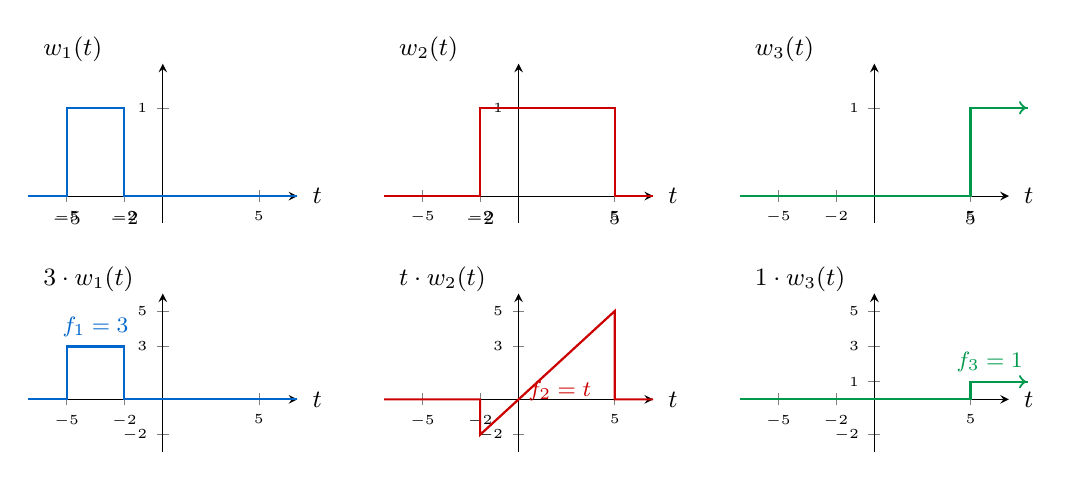
\begin{tikzpicture}
    \begin{groupplot}[
        group style={
            group size=3 by 2,
            horizontal sep=1.1cm,
            vertical sep=0.9cm,
        },
        width=5cm,
        height=3.6cm,
        axis lines=middle,
        xmin=-7, xmax=7,
        ymin=-0.3, ymax=1.5,
        xtick={-5,-2,0,5},
        ytick={0,1},
        xticklabel style={font=\tiny},
        yticklabel style={font=\tiny},
        every axis plot/.append style={thick},
        every axis x label/.append style={at={(ticklabel* cs:1.02)}, anchor=west, font=\small},
        every axis y label/.append style={at={(rel axis cs:0.02,0.95)}, anchor=south west, font=\small},
        tick style={font=\tiny},
    ]

    % ---- FILA 1: VENTANAS ----

    % Ventana 1: [u(t+5) - u(t+2)]
    \nextgroupplot[
        ylabel={$w_1(t)$}, xlabel={$t$},
        extra x ticks={-5,-2},
        extra x tick labels={\scriptsize$-5$, \scriptsize$-2$},
    ]
    \addplot[colorI] coordinates {(-7,0) (-5,0) (-5,1) (-2,1) (-2,0) (7,0)};

    % Ventana 2: [u(t+2) - u(t-5)]
    \nextgroupplot[
        ylabel={$w_2(t)$}, xlabel={$t$},
        extra x ticks={-2,5},
        extra x tick labels={\scriptsize$-2$, \scriptsize$5$},
    ]
    \addplot[colorII] coordinates {(-7,0) (-2,0) (-2,1) (5,1) (5,0) (7,0)};

    % Ventana 3: u(t-5)
    \nextgroupplot[
        ylabel={$w_3(t)$}, xlabel={$t$},
        extra x ticks={5},
        extra x tick labels={\scriptsize$5$},
        clip=false,
    ]
    \addplot[colorIII] coordinates {(-7,0) (5,0) (5,1) (8,1)};
    \draw[->, colorIII, thick] (axis cs:7.5,1) -- (axis cs:7.9,1);

    % ---- FILA 2: FUNCIÓN × VENTANA ----

    % Tramo 1: 3·w1 → constante 3 en [-5, -2]
    \nextgroupplot[
        ymin=-3, ymax=6,
        ytick={-2,0,3,5},
        yticklabel style={font=\tiny},
        ylabel={$3\cdot w_1(t)$}, xlabel={$t$},
    ]
    \addplot[colorI] coordinates {(-7,0) (-5,0) (-5,3) (-2,3) (-2,0) (7,0)};
    \node[colorI, font=\footnotesize, anchor=south] at (axis cs:-3.5,3) {$f_1=3$};

    % Tramo 2: t·w2 → recta t en [-2, 5]
    \nextgroupplot[
        ymin=-3, ymax=6,
        ytick={-2,0,3,5},
        yticklabel style={font=\tiny},
        xmin=-7, xmax=7,
        ylabel={$t\cdot w_2(t)$}, xlabel={$t$},
    ]
    \addplot[colorII] coordinates {(-7,0) (-2,0) (-2,-2) (5,5) (5,0) (7,0)};
    \node[colorII, font=\footnotesize, anchor=west] at (axis cs:0,0.5) {$f_2=t$};

    % Tramo 3: 1·w3 → constante 1 para t>5
    \nextgroupplot[
        ymin=-3, ymax=6,
        ytick={-2,0,1,3,5},
        yticklabel style={font=\tiny},
        ylabel={$1\cdot w_3(t)$}, xlabel={$t$},
        clip=false,
    ]
    \addplot[colorIII] coordinates {(-7,0) (5,0) (5,1) (8,1)};
    \node[colorIII, font=\footnotesize, anchor=south] at (axis cs:6,1) {$f_3=1$};
    \draw[->, colorIII, thick] (axis cs:7.5,1) -- (axis cs:7.9,1);

    \end{groupplot}
\end{tikzpicture}
\end{document}
